\documentclass{article}
\usepackage[utf8]{inputenc}
\usepackage[T1]{fontenc}
\usepackage{lipsum}
\usepackage{graphicx}
\usepackage{amsmath}
\usepackage[margin=1in]{geometry}
\usepackage{titlesec}
\usepackage{graphicx}
\usepackage{floatflt,epsfig}
\usepackage[utf8]{inputenc}
\usepackage[T1]{fontenc}
\usepackage{lipsum}
\usepackage{graphicx}
\usepackage{amsmath}
\usepackage[margin=1in]{geometry} 
\usepackage{titlesec}
\usepackage{listings}
\usepackage{xcolor}
\usepackage{hyperref}
\usepackage{subfigure}
\usepackage{graphicx}

\hypersetup{
    pdfborder = {0 0 0},
}

\lstdefinelanguage{Java}{
  keywords={abstract,assert,boolean,break,byte,case,catch,char,class,const,continue,default,do,double,else,enum,extends,false,final,finally,float,for,goto,if,implements,import,instanceof,int,interface,long,native,new,null,package,private,protected,public,return,short,static,strictfp,super,switch,synchronized,this,throw,throws,transient,true,try,void,volatile,while},
  morekeywords={[2]System,out},
  morecomment=[l]{//},
  morecomment=[s]{/*}{*/},
  morestring=[b]",
  basicstyle=\small\ttfamily,
  keywordstyle=\color{blue}\bfseries,
  keywordstyle={[2]\color{orange}\bfseries},
  commentstyle=\color{green!70!black},
  stringstyle=\color{red},
  showstringspaces=false,
  tabsize=2,
  breaklines=true,
  breakatwhitespace=true,
  frame=single, 
  captionpos=b
}

\titleformat{\section}
{\LARGE\bfseries}{\thesection}{1em}{}

\titleformat{\subsection}
{\Large\bfseries}{\thesection}{1em}{}

\begin{document}

\pagestyle{empty}

\begin{titlepage} 
    \begin{center}
        {{\Large{\textsc{Alma Mater Studiorum - Università di Bologna}}}}
        \rule[0.1cm]{\textwidth}{0.1px}
        \rule[0.5cm]{\textwidth}{0.6px}\\
        {\large{SCUOLA DI SCIENZE \\ Corso di Laurea in Informatica per il Management}}
    \end{center}
    
    \vspace{90px}
    
    \begin{center}
        \LARGE Personal Physical Tracker
    \end{center}
    
    \vspace{100px}
    \par
    \noindent
    \hfill
    \begin{minipage}[t]{0.4\textwidth}\raggedleft
    {\fontsize{12}{13}{}\
    \fontsize{12}{13}{\\ Canghiari Matteo \\ Matricola 1032059 \\ matteo.canghiari@studio.unibo.it}}

    {\fontsize{12}{13}{}\
    \fontsize{12}{13}{\\ Rocca Claudio \\ Matricola 1032059 \\ claudio.rocca@studio.unibo.it}}
    \end{minipage}

    \vspace*{140px}

    \begin{center}
        \large{Laboratorio di Applicazioni Mobili}\\
        \large{Anno Accademico 2023/2024}
    \end{center}
\end{titlepage}

\newpage
\subsection*{Introduzione}
\large

\textbf{Personal Physical Tracker}, è un'applicazione nativa Android che permette all'utente di registrare le attività che compie durante la giornata; le attività registrabili sono la \textbf{camminata}, \textbf{spostamenti in macchina} e \textbf{attività sedentarie}.
L'applicazione si avvale di differenti funzionalità, tra cui la registrazione delle attività compiute e la visualizzazione dei dati di altri utenti presenti sull'applicativo. Tutte le funzionalità presenti saranno successivamente approfondite nella sezione \textbf{Feature}, tuttavia è possibile anticipare ciò che contraddistingue il sistema software ideato. \vspace*{7pt}\\
Ad un primo avvio l'utente visualizzerà una finestra in grado di sovrapporre un frammento di \textit{Login} e di \textit{Sign In}, caratterizzata dai canonici controlli relativi all'\textit{accesso} e \textit{registrazione} dell'applicazione. Proseguendo, verrà mostrato il fulcro dell'app, composto da una \textit{Navigation Bottom Bar}, garantendo in questo modo l'accesso diretto alle funzionalità sviluppate. \\
In questa sezione l'utente avrà la possibilità di \textbf{registrare} nuove attività, \textbf{visualizzare} il proprio storico, osservare le proprie \textbf{aree geografiche di interesse}, visualizzare i \textbf{grafici} relativi alle proprie attività registrate ed, infine, condividere e visualizzare le attività condivise da altri utenti nella sezione \textbf{amici}. \vspace*{7pt}\\
Descritto un breve riepilogo delle peculiarità che possiede l'applicazione, è bene soffermarsi sulle scelte implementative effettuate, in maniera tale da esprimere al meglio il ragionamento dedotto durante lo sviluppo; anche in questa circostanza verranno solamente anticipate alcune tematiche. \vspace*{7pt}\\
Per il versionamento del codice è stato utilizzato \textbf{Git}, con repository accessibile su \textbf{GitHub}, mentre per lo sviluppo dell'applicativo è stato utilizzato il linguaggio di programmazione \textbf{Kotlin}, per la realizzazione di un'applicazione \textbf{nativa Android}. Il progetto si compone di tre strumenti fondamentali per il corretto funzionamento, suddivisi come segue:
\begin{itemize}
    \renewcommand{\labelitemi}{-}
    \item Design pattern architetturale \textbf{MVVM}, adeguato affinchè sia possibile porre un layer aggiuntivo tra il \textit{contenitore statico} di dati, coincidente con il \textbf{Model}, e la sezione \textit{attiva}, definita all'interno della \textbf{View}. In questo modo sono ovviate \textit{dipendenze funzionali}, che potrebbero possedere un effetto distruttivo sull'entità sviluppate, dove piccole modifiche potrebbero compromettere la stabilità del progetto 
    \item \textbf{Room}, utilizzato per garantire la persistenza dei dati all'interno di un \textit{Database Relazionale}
    \item \textbf{Amazon S3}, utilizzato per salvare in cloud i dati degli utenti attraverso un \textit{database dump}, consentendo la condivisione dei dati salvati sul \textit{database locale} e permettendo di visualizzare i dati condivisi dagli amici
\end{itemize}

\newpage
\subsection*{Feature}
\subsubsection*{Feature richieste}
\textit{Registrazione} \vspace*{7pt}\\
All'avvio dell'app è richiesta la registrazione dell'utente, tramite \textit{username} e \textit{password}. E' necessario registrarsi con un username non ancora presente, per garantire l' univocità dei dati. Una volta registrato, all'utente sarà richiesto di concedere tutti i permessi necessari per il funzionamento dell'applicazione.\\
Tra i permessi richiesti sono presenti:
\begin{itemize}
    \renewcommand{\labelitemi}{-}
    \item \textbf{Access fine location}, autorizzazione di accesso alla posizione corrente del dispositivo, necessaria per monitorare le aree geografiche varcate
    \item \textbf{Access background location}, permesso necessario per accedere alla posizione del dispositivo anche quando l'applicazione è in secondo piano
    \item \textbf{Post notifications}, consente di inviare notifiche al dispositivo
\end{itemize}
Qualora siano negati i permessi richiesti sarà comunque consentito di utilizzare l'app, tuttavia le funzionalità che richiedono obbligatoriamente le autorizzazioni saranno disabilitate.
Al riavvio dell'app l'utente può effettuare il login con le stesse credenziali usate in fase di registrazione. \vspace*{7pt}\\
\begin{center}
    \begin{figure}[h]
        \centering
        \subfigure[Immagine 1]{
            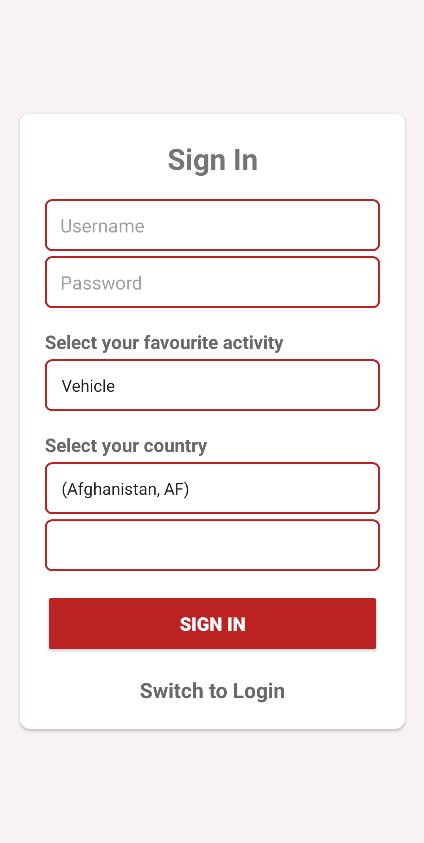
\includegraphics[width=0.35\textwidth]{img1.png}
        }
        \subfigure[Immagine 2]{
            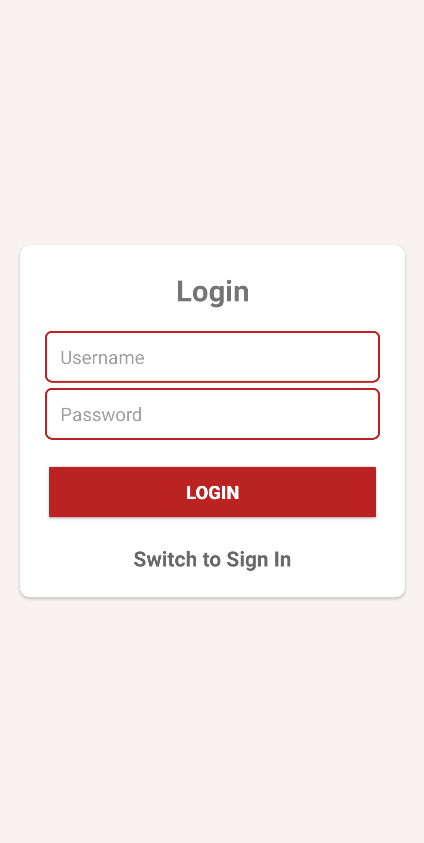
\includegraphics[width=0.35\textwidth]{img2.png}
        }
    \end{figure}
\end{center}
\textit{Registrazione attività} \vspace*{7pt}\\
All'interno dell'app è possibile registrare le attività compiute durante la giornata cliccando sul floating button presente nella schermata Home. L'utente può registrare le seguenti attività:
\begin{itemize}
    \renewcommand{\labelitemi}{-}
    \item \textbf{Attività sedentaria}, in cui viene registrato il tempo trascorso
    \item \textbf{Camminata}, in cui vengono registrati i passi fatti e il dislivello percorso durante l'attività
    \item \textbf{Spostamenti in macchina}, durante i quali viene registrata la distanza percorsa
\end{itemize}
I dati relativi alle attività dell'utente vengono salvati in un database locale e rielaborate per consentire all'utente di visualizzare le attività compiute.
Sulla \textit{homepage} è possibile visualizzare le attività compiute nell'ultimo periodo: l'utente può scegliere se vedere le attività dell'ultimo giorno o dell'ultima settimana, mentre nelle sezioni \textit{calendario} e \textit{grafici}
\newpage
\subsubsection*{Feature aggiuntive}

\subsection*{Scelte implementative}


\subsection*{Possibili sviluppi futuri}



\end{document}
